\documentclass[a4paper,12pt]{article}

\usepackage{mystyle}
\usepackage{gensymb}

\graphicspath{ {images/} }


% https://tex.stackexchange.com/questions/5461/is-it-possible-to-change-the-size-of-an-arrowhead-in-tikz-pgf
\usetikzlibrary{arrows.meta}

% https://tex.stackexchange.com/questions/261591/arrow-above-text-like-widehat
\usepackage{esvect}

% https://tex.stackexchange.com/questions/32501/how-to-get-a-good-divisible-by-symbol
\DeclareRobustCommand{\divby}{%
  \mathrel{\vbox{\baselineskip.65ex\lineskiplimit0pt\hbox{.}\hbox{.}\hbox{.}}}%
}


% Example of color definition:
\definecolor{light-cyan}{RGB}{0, 204, 204}


\author{Алексеев Василий}
\title{Семинар 3}
\date{15 + 20 сентября 2021}


\begin{document}
  \maketitle
  
  \tableofcontents

  \thispagestyle{empty}
  
  \newpage
  
  \pagenumbering{arabic}


  \section{Замена базиса}
  
  \begin{problem}[4.7]
    Есть два базиса на плоскости (которые заданы компонентами в каком-то третьем базисе).
    Первый: $\bds e_1(2, 3)$ и $\bds e_2(3, 4)$.
    Второй: $\bds e_1'(1, -1)$ и $\bds e_2'(2, -3)$.
    
    Надо выразить координаты произвольного вектора $\bds a$ в базисе $\bds e$ по его координатам $(\alpha_1', \alpha_2')$ в базисе $\bds e'$.
  \end{problem}
  
  \begin{solution}
    Обозначим векторы того ``третьего'' базиса (в котором заданы векторы $\bds e$ и $\bds e'$) за $\bds p$ и $\bds q$.
    Занесём в табличку известные координаты участвующих в задаче векторов в разных базисах (\ref{fig:different-basises}).
    
    \begin{table}[h]
      \centering
    
      \caption{Координаты векторов (по вектору в строке) в разных базисах (в столбце~---~координаты векторов в одном базисе). В задаче надо найти \textcolor{light-cyan}{такие} координаты.}
      \label{fig:different-basises}
      
      \begin{tabular}{c|ccc}
        \toprule
        {}          & $(\bds p, \bds q)$ & $(\bds e_1, \bds e_2)$ & $(\bds e_1', \bds e_2')$\\
        \midrule
        $\bds e_1$  & $(2, 3)$           & $(1, 0)$               & $$\\
        $\bds e_2$  & $(3, 4)$           & $(0, 1)$               & $$\\
        \midrule
        $\bds e_1'$ & $(1, -1)$          & $$                     & $(1, 0)$\\
        $\bds e_2'$ & $(2, -3)$          & $$                     & $(0, 1)$\\
        \midrule
        $\bds a$    & $$ & $(\textcolor{light-cyan}{\alpha_1}, \textcolor{light-cyan}{\alpha_2})$ & $(\alpha_1', \alpha_2')$\\
        \bottomrule
      \end{tabular}
    \end{table}
    
    Теперь посмотрим на вектор $\bds a$ в разных базисах:
    \[
      \bds a = \alpha_1 \cdot \bds e_1 + \alpha_2 \cdot \bds e_2
        = \alpha_1' \cdot \bds e_1' + \alpha_2' \cdot \bds e_2'
    \]
    
    Чтобы найти $\alpha_1$ и $\alpha_2$, можно выразить все $\bds e_i$ и $\bds e'_i$ через $\bds p$ и $\bds q$:
    \[
      \alpha_1 \cdot (2 \bds p + 3 \bds q) + \alpha_2 \cdot (3 \bds p + 4 \bds q)
        = \alpha_1' \cdot (\bds p - \bds q) + \alpha_2' \cdot (2 \bds p - 3 \bds q)
    \]

    Тогда после привидения получится, что
    \[
      (2 \alpha_1 + 3 \alpha_2 - \alpha_1' - 2 \alpha_2') \bds p + (3 \alpha_1 + 4 \alpha_2 + \alpha_1' + 3 \alpha_2') \bds q = \bds 0
    \]
    линейная комбинация векторов $\bds p$ и $\bds q$ равна нулю.
    Но, так как они линейно независимые, отсюда можно заключить, что нулю равны коэффициенты при $\bds p$ и $\bds q$:
    \[
      \left\{
        \begin{aligned}
          &2 \alpha_1 + 3 \alpha_2 - \alpha_1' - 2 \alpha_2' = 0\\
          &3 \alpha_1 + 4 \alpha_2 + \alpha_1' + 3 \alpha_2' = 0
        \end{aligned}
      \right.
    \]
  
  Решая полученную систему (например, с помощью правила Крамера), получаем:
  \[
    \left\{
      \begin{aligned}
        &\alpha_1 = -7 \alpha_1' - 17 \alpha_2'\\
        &\alpha_2 = 5 \alpha_1' + 12 \alpha_2'
      \end{aligned}
    \right.
  \]
  \end{solution}
  
  Решённая задача~---~пример перехода от одного базиса к другому.
  Рассмотрим этот вопрос в более общем виде.
  Будем обозначать векторы базиса в виде строки.
  Например:
  \[
    \bds e \hm= (\bds e_1, \bds e_2, \bds e_3)
  \]
  для случая базиса во всём пространстве $\RR^3$.
  Аналогично и для базисов на плоскости и на прямой (в $\RR^2$ и в $\RR$).
  
  При заданном базисе $\bds e$ любой вектор $\bds a$ пространства однозначно определяется его компонентами в базисе:
  \[
    \bds a = x_1 \cdot \bds e_1 + x_2 \cdot \bds e_2 + x_3 \cdot \bds e_3
      \Rightarrow \bds a \leftrightarrow \bds x = (x_1, x_2, x_3)^T
  \]
  поэтому, говоря о векторе~---~направленном отрезке, часто имеют в виду его компоненты в базисе (то есть понятия вектора как направленного отрезка и вектора как столбца из чисел при фиксированном базисе взаимозаменяемы).
  
  В пространстве существует больше одного базиса: любая тройка некомпланарных векторов в $\RR^3$ образует базис.
  Встаёт вопрос о том, как связаны компоненты одного и того же вектора в разных базисах.
  
  \begin{figure}[h]
    \centering
    
    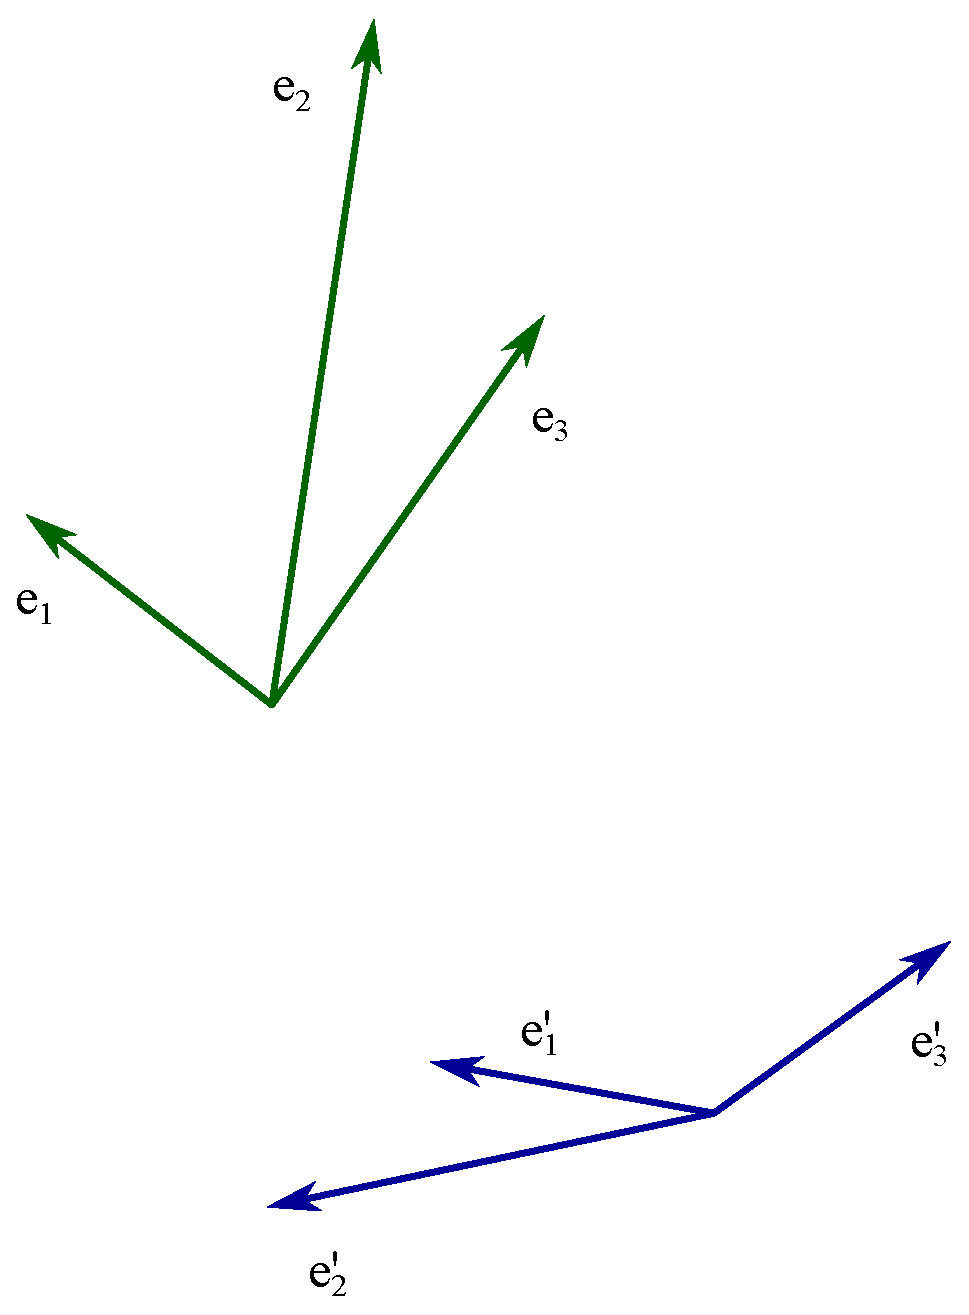
\includegraphics[width=0.5\columnwidth]{two-basises}
    
    \caption{Два разных базиса в пространстве.}
    \label{fig:two-basises}
  \end{figure}
  
  Пусть есть два базиса: $\bds e$ и $\bds e'$ (\ref{fig:two-basises}).
  Тогда векторы базиса $\bds e'$ можно разложить по $\bds e$:
  \begin{equation}\label{eq:e1-to-e2-via-system-of-equations}
    \left\{
      \begin{aligned}
        &\bds e_1' = a_{11} \cdot \bds e_1 + a_{12} \cdot \bds e_2 + a_{13} \cdot \bds e_3\\
        &\bds e_2' = a_{21} \cdot \bds e_1 + a_{22} \cdot \bds e_2 + a_{23} \cdot \bds e_3\\
        &\bds e_3' = a_{31} \cdot \bds e_1 + a_{32} \cdot \bds e_2 + a_{33} \cdot \bds e_3
      \end{aligned}
    \right.
  \end{equation}
  
  Запись можно представить более компактно\footnote{Под результатом умножения строки из векторов $\bds e$ на матрицу из чисел $S$ будем иметь в виду такую строку $\bds e'$ из векторов, где каждый элемент равен линейной комбинации векторов умножаемой строки $\bds e$ с коэффициентами, равными элементам соответственного столбца матрицы $S$. То есть по правилу умножения числовых матриц.}:
  \[
    \bds e' = \bds e S
  \]
  где $S$ называется \emph{матрицей перехода} от базиса $\bds e$ (``старого'') к базису $\bds e'$ (``новому''):
  \[
    S = \begin{pmatrix}
      a_{11} & a_{21} & a_{31}\\
      a_{12} & a_{22} & a_{32}\\
      a_{13} & a_{23} & a_{33}
    \end{pmatrix}
  \]
  во введённых ранее обозначениях (\ref{eq:e1-to-e2-via-system-of-equations}).
  Столбцы матрицы перехода $S$~---~это координаты векторов нового базиса в старом базисе (``переход от $\bds e$ к $\bds e'$'': зная векторы $\bds e$, надо получить векторы $\bds e'$).
  
  Посмотрим теперь, как выражаются компоненты некоторого вектора $\bds a$ в одном базисе через его же компоненты, но в другом базисе.
  Имеем
  \begin{equation}\label{eq:same-vector-two-faces}
    \bds a = \bds e \bds x = \bds e' \bds x'
  \end{equation}
  где $\bds a$~---~вектор как направленный отрезок,
  $\bds x \hm\equiv \bds x_e$~---~вектор-столбец, соответствующий $\bds a$ в базисе $\bds e$,
  $\bds x' \hm\equiv \bds x_{e'}$~---~вектор-столбец, соответствующий $\bds a$ в базисе $\bds e'$.
  
  Теперь воспользуемся тем, что нам известно представление базиса $\bds e'$ через вектора базиса $\bds e$:
  \[
    \bds e' \bds x' = \bigl(\bds e S\bigr) \bds x'
      \stackrel{(\ref{eq:same-vector-two-faces})}{=} \bds e \bds x
  \]
  Так как умножение матриц ассоциативно, а также дистрибутивно относительно матричного сложения, мы можем перенести $\bds e \bds x$ влево и перегруппировать слагаемые:
  \[
    \bds e \cdot \bigl(S \bds x' - \bds x\bigr) = \bds 0
  \]
  
  Из линейной независимости системы векторов $\bds e$ получаем:
  \[
    S \bds x' - \bds x = \bds 0 \Leftrightarrow \bds x = S \bds x'
  \]
  
  Итак, в двух базисах компоненты векторов связаны так:
  \begin{equation}\label{eq:vector1-to-vector2}
    \boxed{
      \left\{
        \begin{aligned}
          &\bds e' = \bds e S\\
          &\bds x = S \bds x'
        \end{aligned}
      \right.
    }
  \end{equation}
  
  При этом, при переходе, наоборот, от базиса $\bds e'$ к базису $\bds e$ можно написать аналогичное соотношение, но уже с другой матрицей перехода, которую обозначим за $S'$:
  \[
    \left\{
      \begin{aligned}
        &\bds e = \bds e' S'\\
        &\bds x' = S' \bds x
      \end{aligned}
    \right.
  \]
  
  
  \subsection{Поворот базиса}
  
  Рассмотрим отдельно преобразование поворота правого\footnote{Поворот от первого базисного вектора ко второму по наименьшему углу происходит против часовой стрелки.} ортонормированного базиса $\bds e_1, \bds e_2$ на плоскости на угол $\phi$ против часовой стрелки (\ref{fig:turned-ortonorm-basis}).

  \begin{figure}[h]
    \centering
    
    \includegraphics[width=0.4\columnwidth]{turned-ortonorm-basis}
    
    \caption{Базис $\bds e'$ повёрнут на угол $\phi$ относительно базиса $\bds e$.}
    \label{fig:turned-ortonorm-basis}
  \end{figure}
  
  Имеем для компонент векторов $\bds e'$ в базисе $\bds e$\footnote{Угол именно $\phi + \frac{\pi}{2}$! чтобы при умножении на $\cos$/$\sin$ получить скалярные проекции на направления базисных векторов.}:
  \[
    \left\{
      \begin{aligned}
        &\bds e_1' = |\bds e_1'| \cdot \cos\phi \cdot \bds e_1 + |\bds e_1'| \cdot \sin\phi \cdot \bds e_2\\
        &\bds e_2' = |\bds e_2'| \cdot \cos{\left(\phi + \frac{\pi}{2}\right)} \cdot \bds e_1 + |\bds e_2'| \cdot \sin{\left(\phi + \frac{\pi}{2}\right)} \cdot \bds e_2
      \end{aligned}
    \right.
  \]
  
  Так как модули векторов единичные:
  \[
    \bds e' = \bds e \begin{pmatrix}
      \cos\phi & \cos{\left(\phi + \frac{\pi}{2}\right)}\\
      \sin\phi & \sin{\left(\phi + \frac{\pi}{2}\right)}
    \end{pmatrix}
  \]
  
  То есть матрица перехода:
  \[
    S' = \begin{pmatrix}
      \cos\phi & \cos{\left(\phi + \frac{\pi}{2}\right)}\\
      \sin\phi & \sin{\left(\phi + \frac{\pi}{2}\right)}
    \end{pmatrix}
    = \begin{pmatrix}
      \cos\phi & -\sin\phi\\
      \sin\phi & \cos\phi
    \end{pmatrix}
  \]
  
  Таким образом, получили матрицу, задающую поворот правого ортонормированного базиса на угол $\phi$ против часовой стрелки.
  То же самое получилось бы, если бы старый базис был левый ортонормированный, а новый получался бы его поворотом по часовой стрелке на угол $\phi$.
  
  Аналогично можно получить матрицу перехода, когда базис $\bds e'$ не только повёрнут относительно $\bds e$, но если второй вектор ещё отражён относительно первого.
  То есть если базис $\bds e'$ левый, а $\bds e$ правый, и наоборот (\ref{fig:turned-ortonorm-basis2}).
  В этом случае при нахождении $\bds e_2'$ будет использоваться угол не $\phi \hm+ \dfrac{\pi}{2}$, а $\phi \hm- \dfrac{\pi}{2}$.
  
  \begin{figure}
    \centering
    
    \begin{subfigure}[b]{0.3\columnwidth}
      \centering
      \includegraphics[width=\textwidth]{turned-ortonorm-basis2_left2}
      \caption{$\bds e$ правый, а $\bds e'$ левый.}
    \end{subfigure}
    \hspace{5em}
    \begin{subfigure}[b]{0.4\columnwidth}
      \centering
      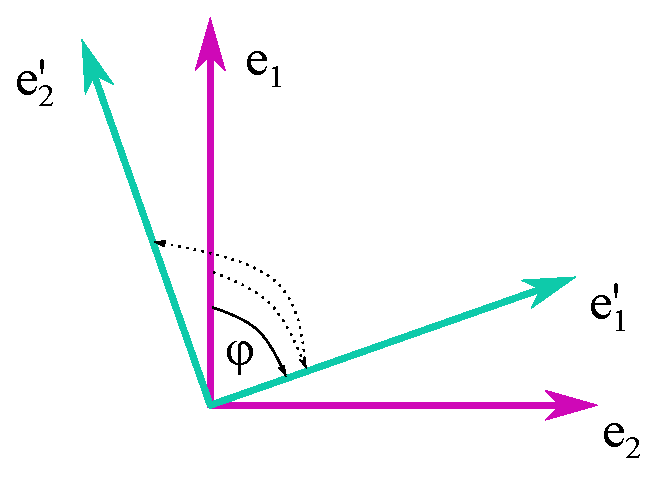
\includegraphics[width=\textwidth]{turned-ortonorm-basis2_left1}
      \caption{$\bds e$ левый, а $\bds e'$ правый.}
    \end{subfigure}  % TODO: make axes of plots equal
    
    \caption{Базис $\bds e'$ повёрнут на угол $\phi$ относительно базиса $\bds e$, при этом поворот от первого вектора ко второму по наименьшему углу в старом и новом базисах совершается в разные стороны.}
    \label{fig:turned-ortonorm-basis2}
  \end{figure}


  \section{Система координат $+$ Замена}
  
  Имея базис в пространстве, можно описать любой вектор с помощью столбца из чисел~---~его координат в базисе.
  Но как описать просто точку?
  Ведь у неё нет ни ``длины'', ни ``направления''...
  Один из способов~---~зафиксировать некоторую точку $O$, и строить векторы с началом в $O$ и концом в интересующей точке пространства (\emph{радиусы-векторы}).
  Тогда за описание точки можно принять координаты соответствующего ей радиуса-вектора (при выбранном базисе и выбранной точке $O$).
  Описанный способ задания точек называется \emph{общей декартовой системой координат}\footnote{Помимо декартовой, есть и другие системы координат. Например полярная, когда положение точки на плоскости определяется по расстоянию $r$ от начала координат $O$ и по углу $\phi$, которое направление из начала координат на точку образует с выбранным направлением $\bds l$: $\bds a \hm\leftrightarrow (r, \phi)$.} (\ref{fig:coord-system}).
  
  \begin{figure}[h]
    \centering
    
    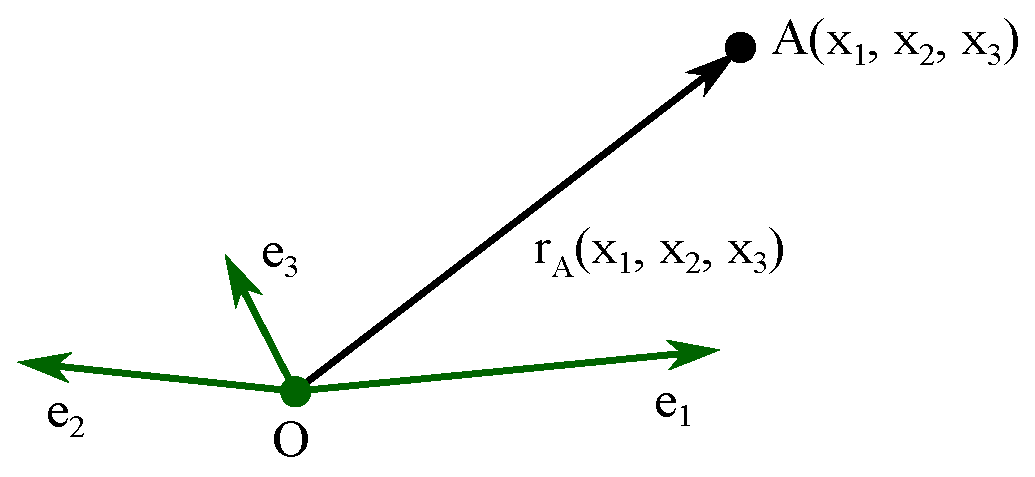
\includegraphics[width=0.5\columnwidth]{coord-system}
    
    \caption{Общая декартова система координат (совокупность точки и базиса)~---~способ описания точек в пространстве.}
    \label{fig:coord-system}
  \end{figure}
  
  \begin{definition}
    Общей декартовой системой координат называется совокупность точки $O$ (\emph{начала системы координат}) и базиса: $(O; \bds e_1, \ldots, \bds e_n)$
  \end{definition}
  
  \begin{definition}
    Прямоугольной декартовой системой координат называется такая общая декартова система координат, в которой базисные векторы перпендикулярны и по длине равны единице.
  \end{definition}
  
  \begin{remark}
    При заданной системе координат $O; \bds e_1, \ldots, \bds e_n$ каждой точке $A$ можно поставить в соответствие набор чисел~---~компонент радиуса-вектора точки в базисе $\vv{OA} \hm= \alpha_1 \bds e_1 \hm+ \ldots \hm+ \alpha_n \bds e_n$:
    \[
      A \leftrightarrow (\alpha_1, \ldots, \alpha_n) \in \RR^n
    \]
  \end{remark}

  \begin{figure}[H]
    \centering
    
    \includegraphics[width=0.5\columnwidth]{two-coords}
    
    \caption{Две системы координат в пространстве.}
    \label{fig:two-coords}
  \end{figure}

  Аналогично с заменой базиса, может возникнуть вопрос, как меняются координаты точек при смене системы координат (\ref{fig:two-coords}).
  Пусть есть две системы координат: ``старая'' $(O; \bds e)$ и ``новая'' $(O'; \bds e')$.
  Пусть нам известно положение точки $A$ относительно новой системы координат.
  Также пусть нам известно, как выражаются базисные векторы новой системы $\bds e'$ через векторы старой $\bds e$ и как расположено начало новой системы $O'$ в старой системе.
  Очевидно, по этой информации мы должны уметь найти, как расположена точка $A$ в старой системе координат $(O; \bds e)$...
  
  Введём обозначения: пусть $\bds r_A \hm\equiv \bds r_O(A)$~---~радиус-вектор точки $A$ в системе $(O; \bds e)$,
  $\bds r'_A \hm\equiv \bds r_{O'}(A)$~---~радиус-вектор точки $A$ в системе $(O'; \bds e')$,
  и $\bds r_{O'} \hm\equiv \bds r_O(O')$~---~радиус-вектор, определяющий положение начала отсчёта $O'$ в системе $(O; \bds e)$.
  Очевидно, что
  \[
    \bds r_A = \bds r_{O'} + \bds r'_A
  \]
  
  В системе $(O'; \bds e')$ известно координатное представление вектора $\bds r'_A$.
  Для вектора $\bds r_{O'}$ известны компоненты в базисе $(O; \bds e)$.
  Как записать соотношение выше через вектор-столбцы компонент векторов в базисах?
  Для этого \emph{надо все векторы представить в одном базисе}.
  Из соотношений (\ref{eq:vector1-to-vector2}) мы можем найти вектор-столбец радиуса-вектора $\bds r'_A$ в базисе $\bds e$ по его координатному столбцу $\bds x'_A$ в базисе $\bds e'$.
  Он будет равен $S \bds x'_A$.
  Итого, получаем соотношение для компонент радиусов-векторов точки в разных системах координат:
  \begin{equation}\label{eq:point1-to-point2}
    \boxed{
      \left\{
        \begin{aligned}
          &\bds e' = \bds e S\\
          &\bds x_A = \bds x_{O'} + S \bds x'_A
        \end{aligned}
      \right.
    }
  \end{equation}
  то есть для нахождения координат точки в ``старой'' системе по её координатам в ``новой'' системе координат надо знать, как выражаются векторы ``новой'' системы в базисе ``старой'' и как расположено начало координат ``новой'' системы в ``старой''.

  \begin{problem}[4.19]
    Треугольная призма $A B C A_1 B_1 C_1$ (\ref{fig:prism}).
    Точка $M$~---~точка пересечения медиан грани $A_1 B_1 C_1$.
    Требуется, зная координаты точки $x', y', z')$ в системе $A_1; \vv{A_1 B}, \vv{A_1 C}, \vv{A_1 M}$, найти её координаты $(x, y, z)$ в системе $A; \vv{AB}, \vv{AC}, \vv{AB_1}$\footnote{Порядок базисных векторов важен!}.
    \begin{figure}[h]
      \centering
    
      \includegraphics[width=0.5\columnwidth]{prism}
    
      \caption{Призма $ABC A_1 B_1 C_1$.}
      \label{fig:prism}
    \end{figure}
  \end{problem}
  
  \begin{solution}
    Что нам надо найти?
    Вспоминая формулы (\ref{eq:vector1-to-vector2}) или (\ref{eq:point1-to-point2}), получаем, что если векторы базиса связаны соотношением $\bds e' \hm= \bds e S$, то компоненты векторов связаны соотношением $\bds x \hm= S \bds x'$ и координаты точек связаны соотношением $\bds x \hm= \bds x_{O'} \hm+ S \bds x'$.
    Таким образом, чтобы решить задачу, надо найти матрицу $S$, столбцы которой~---~компоненты базиса $\vv{A_1 B}, \vv{A_1 C}, \vv{A_1 M}$ в базисе $\vv{AB}, \vv{AC}, \vv{AB_1}$, и координаты начала $A_1$ в системе с началом $A$.
    Обозначим $\vv{AB}, \vv{AC}, \vv{AB_1}$ за $\bds e_1, \bds e_2, \bds e_3$ и разложим $\vv{A_1 B}, \vv{A_1 C}, \vv{A_1 M}$ по этой системе:
    \[
      \vv{A_1 B} = \vv{A_1 A} + \vv{AB} = \vv{A_1 B_1} + \vv{B_1 A} + \vv{AB} = \bds e_1 - \bds e_3 + \bds e_1
    \]
    \[
      \vv{A_1 C} = \vv{A_1 A} + \vv{AC} = \vv{A_1 B_1} + \vv{B_1 A} + \vv{AC} = \bds e_1 - \bds e_3 + \bds e_2
    \]
    \[
      \vv{A_1 M} = \frac{2}{3} \cdot \frac{1}{2} (\vv{A_1 A_1} + \vv{A_1 B_1} + \vv{A_1 C_1}) = \frac{1}{3} (\vv{AB} + \vv{AC})
        = \frac{1}{3} (\bds e_1 + \bds e_2)
    \]
    
    Итого,
    \[
      (\bds e_1', \bds e_2', \bds e_3') = (\bds e_1, \bds e_2, \bds e_3) \begin{pmatrix}
        2 & 1 & 1/3\\
        0 & 1 & 1/3\\
        -1 & -1 & 0
      \end{pmatrix}
    \]
    
    Положение $A_1$ в системе $(A; \bds e)$:
    \[
      \vv{AA_1} = \vv{AB_1} + \vv{B_1 A_1} = \bds e_3 - \bds e_1
    \]
    
    Поэтому связь между координатами точек в разных системах:
    \[
      \bds x = \begin{pmatrix}
        2 & 1 & 1/3\\
        0 & 1 & 1/3\\
        -1 & -1 & 0
      \end{pmatrix} \bds x'
      + \begin{pmatrix}
        -1\\
        0\\
        1
      \end{pmatrix}
    \]
  \end{solution}
  

  
  \section{Дополнение}
  
  \subsection{Скалярное произведение}
  
  \begin{definition}
    Скалярное произведение $(\bds a, \bds b)$ ненулевых векторов $\bds a$ и $\bds b$ определяется следующим образом:
    \begin{equation}
      (\bds a, \bds b) \equiv |\bds a| \cdot |\bds b| \cdot \cos \phi
    \end{equation}
    где $|\bds a|$ и $|\bds b|$~---~модули векторов $\bds a$ и $\bds b$,
    а $\phi$~---~угол между векторами $\bds a$ и $\bds b$ (не превосходящий $\pi$).
    В случае, если хотя бы один из пары векторов нулевой, скалярное произведение этих векторов полагается равным нулю.
  \end{definition}
  
  Отметим несколько свойств скалярного произведения:
  \begin{itemize}
    \item $(\bds a, \bds b) = (\bds b, \bds a)$~---~симметричность
    \item $(\bds a, \bds a) = |\bds a|^2$~---~скалярный квадрат вектора равен квадрату его длины
    \item О равенстве нулю скалярного произведения:
      \[
        (\bds a, \bds b) = 0 \Leftrightarrow \bds a = 0\ \mbox{или}\ \bds b = 0\ \mbox{или}\ \bds a \perp \bds b
      \]
    \item Линейность по первому аргументу:
      \[
        (\alpha \bds a + \beta \bds b, \bds c) = \alpha (\bds a, \bds c) + \beta (\bds b, \bds c)
      \]
  \end{itemize}
  
  Первые три свойства следуют из определения.
  Докажем последнее свойство.
  
  \begin{figure}[h]
    \centering
    
    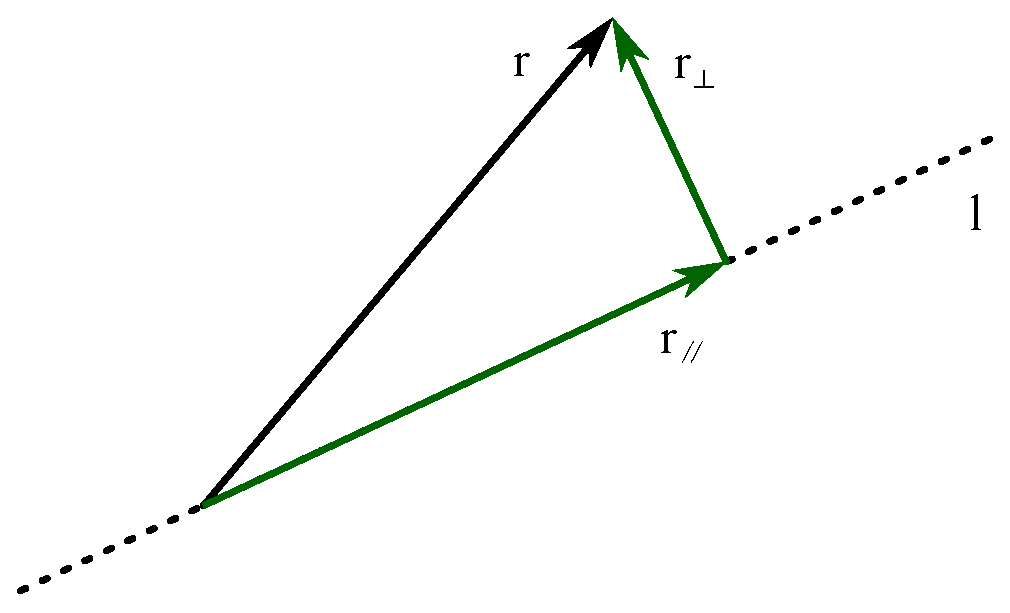
\includegraphics[width=0.5\columnwidth]{vector-projection}
    
    \caption{Векторная проекция вектора $\bds r$ на направление, определяемое вектором $\bds l$.}
    \label{fig:vector-projection}
  \end{figure}
  
  Начнём с того, что при заданном направлении $\bds l$ любой вектор раскладывается в сумму двух (\ref{fig:vector-projection}):
  \[
    \bds r = \bds r_{\parallel} + \bds r_{\perp}
  \]
  где $\bds r_{\parallel}$~---~вектор, параллельный $\bds l$, и $\bds r_{\perp}$~---~вектор, перпендикулярный $\bds l$.
  Компонента $\bds r_{\parallel}$ называется \emph{ортогональной векторной проекцией} вектора $\bds r$ на направление, определяемое вектором $\bds l$, и может обозначаться так:
  \[
    \pi_{\bds l}(\bds r) \equiv \bds r_{\parallel}
  \]
  
  Кроме векторной проекции, есть ещё понятие скалярное проекции вектора $\bds r$ на направление вектора $\bds l$:
  \[
    \pi_{\bds l}(\bds r) \equiv |\bds r_{\parallel}| \cdot \left\{
      \begin{aligned}
        &+1 & &\mbox{если $\bds r_{\parallel} \upuparrows \bds l$}\\
        &-1 & &\mbox{если $\bds r_{\parallel} \updownarrows \bds l$}
      \end{aligned}
    \right.
  \]
  
  Будем обозначать векторную и скалярную проекции одинаково.
  Но из контекста будет понятно, какая имеется в виду.

  Спроецируем теперь вектор $\alpha \bds a \hm+ \beta \bds b$ на направление, определяемое вектором $\bds c$:
  \[
    \pi_{\bds c}(\alpha \bds a + \beta \bds b) = |\alpha \bds a + \beta \bds b| \cdot \cos \phi
  \]
  где $\pi_{\bds c}(\cdot)$~---~скалярная проекция на направление вектора $\bds c$,
  $\phi$~---~угол между вектором $\alpha \bds a \hm+ \beta \bds b$ и вектором $\bds c$.
  Но проекция вектора, являющегося суммой нескольких векторов, равна сумме проекций этих векторов\footnote{В силу линейности скалярного произведения.}:
  \[
    \pi_{\bds c}(\alpha \bds a + \beta \bds b) = \pi_{\bds c}(\alpha \bds a) + \pi_{\bds c}(\beta \bds b)
  \]
  поэтому
  \[
    |\alpha \bds a + \beta \bds b| \cdot \cos \phi = |\alpha \bds a| \cdot \cos \phi_1 + |\beta \bds b| \cdot \cos \phi_2
  \]
  где $\phi_1$ и $\phi_2$~---~углы, которые образуют векторы $\alpha \bds a$ и $\beta \bds b$ с вектором $\bds c$.
  Умножая обе части последнего равенства на модуль вектора $\bds c$, получаем то, что хотели доказать (при этом числовые множители можно вынести за знак модуля):
  \[
    (\alpha \bds a + \beta \bds b, \bds c) = \alpha (\bds a, \bds c) + \beta (\bds b, \bds c)
  \]
  \qed
  
  
  \begin{problem}[2.21]
    Длины базисных векторов $\bds e_1, \bds e_2, \bds e_3$ равны соответственно $3, \sqrt{2}$ и $4$.
    Углы между векторами $\angle (\bds e_1, \bds e_2) \hm= \angle (\bds e_2, \bds e_3) \hm= 45\degree$, $\angle (\bds e_1, \bds e_3) \hm= 60\degree$.
    
    Надо найти длины сторон и углы параллелограмма, построенного на векторах с координатами $(1, -3, 0)$ и $(-1, 2, 1)$ в указанном базисе.
  \end{problem}
  
  \begin{solution}
    Обозначим данные нам векторы за $\bds a$ и $\bds b$:
    \[
      \left\{
        \begin{aligned}
          &\bds a = (1, -3, 0)\\
          &\bds b = (-1, 2, 1)
        \end{aligned}
      \right.
    \]
    
    Базис не ортонормированный, поэтому скалярные произведения надо будет считать ``по-честному''.
    
    Модуль вектора $\bds a$:
    \[
      |\bds a| = \sqrt{(\bds a, \bds a)} = \sqrt{(\bds e_1 - 3\bds e_2)(\bds e_1 - 3\bds e_2)}
        = \sqrt{(\bds e_1, \bds e_1) - 6(\bds e_1, \bds e_2) + 9(\bds e_2, \bds e_2)}
        = \sqrt{9 - 18 + 18} = 3
    \]
    
    Аналогично для вектора $\bds b$:
    \[
      |\bds b| = \sqrt{(\bds b, \bds b)} = \sqrt{(-\bds e_1 + 2\bds e_2 + \bds e_3)(-\bds e_1 + 2\bds e_2 + \bds e_3)}
        = \ldots = 5
    \]
    
    Косинус угла между векторами $\bds a$ и $\bds b$:
    \[
      \cos\angle(\bds a, \bds b) = \frac{(\bds a, \bds b)}{|\bds a| \cdot |\bds b|}
        = \frac{(\bds e_1 - 3\bds e_2) \cdot (-\bds e_1 + 2\bds e_2 + \bds e_3)}{3 \cdot 5}
        = \ldots = -\frac{12}{15} = -\frac{4}{5}
    \]
    
    И острый угол параллелограмма можно найти как $\arccos{\left(\dfrac{4}{5}\right)}$.
  \end{solution}
  
  В случае же \textbf{ортонормированного} базиса формулы с применением скалярных произведений упрощаются:
  \[
    (\bds a, \bds b) = \sum_{i=1}^n a_i b_i
  \]
  \[
    |\bds a| = \sqrt{\sum_{i=1}^n a_i^2}
  \]
  \[
    \cos\angle(\bds a, \bds b) = \frac{\sum_{i=1}^n a_i b_i}{\sqrt{\sum_{i=1}^n a_i^2} \sqrt{\sum_{i=1}^n b_i^2}}
  \]
  
  
  
  
  \subsection{Ещё пара задач про несколько систем координат}
  
  \begin{problem}[4.23]
    Пусть $(x, y)$~---~координаты точки в некоторой прямоугольной системе координат $(O; \bds e)$, а $(x', y')$~---~координаты той же точки в некоторой другой системе координат $(O'; \bds e')$.
    При этом
    \[
      \left\{
        \begin{aligned}
          &x = a_{11} x' + a_{12} y' + a_{10}\\
          &y = a_{21} x' + a_{22} y' + a_{20}
        \end{aligned}
      \right.
    \]
    
    При каком необходимом и достаточном условии вторая система координат $(O'; e')$ также будет прямоугольной?
  \end{problem}
  
  \begin{solution}
    Итак, если переписать связь между координатами точки в разных системах координат в матричном виде
    \[
      \bds x = S \bds x' + \bds x_{O'}
    \]
    где
    \[
      \left\{
        \begin{aligned}
          &S = \begin{pmatrix}
              a_{11} & a_{12}\\
              a_{21} & a_{22}
            \end{pmatrix}\\
          &\bds x_{O'} = \begin{pmatrix}
              a_{10}\\ a_{20}
            \end{pmatrix}
        \end{aligned}
      \right.
    \]
    
    Тогда связь между базисами
    \[
      \bds e' = \bds e S
    \]
    \[
      (\bds e_1', \bds e_2') = \begin{pmatrix}
        a_{11} \bds e_1 + a_{21} \bds e_2
        & a_{12} \bds e_1 + a_{22} \bds e_2
      \end{pmatrix}
    \]
    
    То, что $\bds e$ прямоугольный, означает, что
    \[
      \left\{
        \begin{aligned}
          &(\bds e_i, \bds e_i) = 1\\
          &(\bds e_i, \bds e_j) = 0,\ i \not= j
        \end{aligned}
      \right.
    \]
    
    Выпишем аналогичные условия для базиса $\bds e'$:
    \[
      \left\{
        \begin{aligned}
          &(\bds e_1', \bds e_1') = a_{11}^2 \bds e_1^2 + a_{21}^2 \bds e_2^2 = 1\\
          &(\bds e_2', \bds e_2') = a_{12}^2 \bds e_1^2 + a_{22}^2 \bds e_2^2 = 1\\
          &(\bds e_1', \bds e_2') = a_{11} a_{12} \bds e_1^2 + a_{21} a_{22} \bds e_2^2 = 0
        \end{aligned}
      \right.
    \]
    
    И в итоге:
    \[
      \left\{
        \begin{aligned}
          &a_{11}^2 + a_{21}^2 = 1\\
          &a_{12}^2 + a_{22}^2 = 1\\
          &a_{11} a_{12} + a_{21} a_{22} = 0\\
        \end{aligned}
      \right.
    \]
    
    Можно заметить, что матрицы $S$ вида
    \[
      S = \begin{pmatrix}
        \cos \phi & \mp \sin \phi\\
        \sin \phi & \pm \cos \phi
      \end{pmatrix}
    \]
    удовлетворяют полученным соотношениям.
    Действительно, так как базисы $\bds e$ и $\bds e'$ оба прямоугольные, то один переводится в другой с помощью поворота или отражения\footnote{По знаку определителя матрицы $S$ можно сказать о том, какое именно преобразование связывает два базиса: только поворот (при котором направление поворота от $\bds e_1'$ к $\bds e_2'$ по наименьшему углу совпадает с направлением поворота по наименьшему углу от $\bds e_1$ к $\bds e_2$) или ещё и отражение одного базисного вектора относительно другого (когда меняется \emph{класс базиса}).}.
  \end{solution}
  
  
  \begin{problem}[4.30]
    Пусть $(O; \bds e)$ и $(O'; \bds e')$~---~две прямоугольные системы координат в пространстве $\RR^3$.
    При этом точки $O$ и $O'$ различны, а концы векторов $\bds e_i$ и $\bds e_i'$, отложенных из точек $O$ и $O'$ соответственно, совпадают ($i = 1, 2, 3$).
    Найти координаты точки $(x, y, z)$ в первой системе, зная её координаты во второй системе $(x', y', z')$.
  \end{problem}
  
  \begin{solution}
    \begin{figure}[h]
      \centering
    
      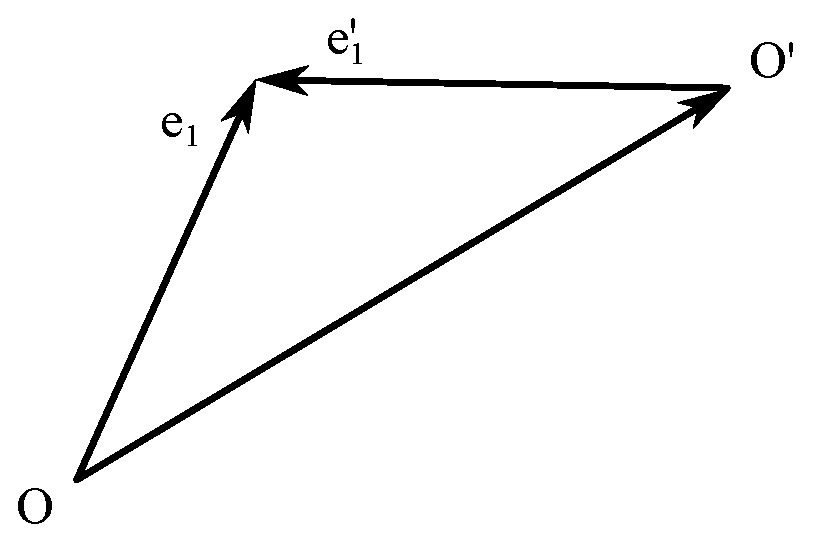
\includegraphics[width=0.5\columnwidth]{two-vectors-kiss}
    
      \caption{Концы соответственных базисных векторов, отложенных от соответствующих начал координат, совпадают.}
      \label{fig:two-vectors-kiss}
    \end{figure}
    
    Условие о том, что концы базисных векторов совпадают (при условии, что векторы отложены из начал систем координат), можно записать так (\ref{fig:two-vectors-kiss})
    \[
      \bds e_i = \vv{OO'} + \bds e_i'
    \]
    
    Нужно найти преобразование
    \[
      \bds x = S \bds x' + \bds x_{O'}
    \]
    
    В то же время
    \[
      \bds e' = \bds e S
    \]
    
    Поэтому матрицу $S$ можно записать так
    \[
      S = \begin{pmatrix}
        \begin{pmatrix}1\\ 0\\ 0\end{pmatrix} - \vv{OO'}_{\bds e}
        & \begin{pmatrix}0\\ 1\\ 0\end{pmatrix} - \vv{OO'}_{\bds e}
        & \begin{pmatrix}0\\ 0\\ 1\end{pmatrix} - \vv{OO'}_{\bds e}
      \end{pmatrix}
    \]
    где $\vv{OO'}_{\bds e}$~---~компоненты вектора $\vv{OO'}$ в базисе $\bds e$ (то же самое, что и $\bds x_{O'}$ в формуле, связывающей координаты точек).
    
    Получается, осталось лишь найти $\vv{OO'}$ в базисе $\bds e$.
    Это можно сделать, потому что мы учли ещё не всю информацию о взаимном расположении систем координат.
    На самом деле тот факт, что обе системы координат прямоугольные и концы соответственных векторов, отложенных из начал соответствующих систем координат, совпадают, означает, что у нас есть ``два поставленных друг на друга прямоугольных тетраэдра'' (\ref{fig:many-vectors-kisses}).
    
    \begin{figure}[h]
      \centering
    
      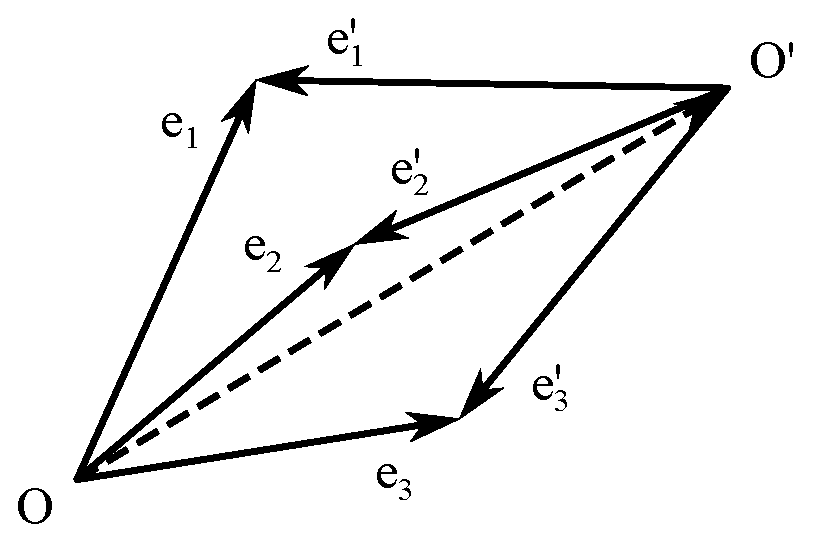
\includegraphics[width=0.5\columnwidth]{many-vectors-kisses}
    
      \caption{Базисы, отложенные от соответствующих начал координат~---~прямоугольные тетраэдры.}
      \label{fig:many-vectors-kisses}
    \end{figure}  % TODO: kisses should not be on the same line
    
    Поэтому вектор $\vv{OO'}$ можно найти как
    \[
      \vv{OO'} = 2 \cdot \left(\frac{1}{3} \bds e_1 + \frac{1}{3} \bds e_2 + \frac{1}{3} \bds e_3\right)
    \]
    (так как проекция точки пересечения $OO'$ с плоскостью концов базисных векторов на грани векторов $\bds e_i, \bds e_j$ совпадает с точкой пересечения медиан треугольников соответствующих граней\footnote{Точка $P$ пересечения $OO'$ с плоскостью концов базисных векторов $E_1 E_2 E_3$~---~очевидно, точка пересечения медиан $\triangle E_1 E_2 E_3$. То есть его центр масс. Если ``двигать'' одну из вершин $\triangle E_1 E_2 E_3$ по нормали до пересечения с гранью тетраэдра, скажем, двигать $E_3$ по нормали к плоскости $O E_1 E_2$, то она окажется вершиной $O$ при прямом угле в $\triangle O E_1 E_2$, а $P$ перейдёт в центр масс прямоугольного треугольника $O E_1 E_2$. Но положение проекции $P$ на грань $O E_1 E_2$ не менялось при сдвиге вершины $E_3$ по нормали к $O E_1 E_2$.}).
    
    Тогда матрица $S$ равна
    \begin{equation}
    \begin{split}
      S &= \begin{pmatrix}
        \begin{pmatrix}1\\ 0\\ 0\end{pmatrix} - \begin{pmatrix}2/3\\ 2/3\\ 2/3\end{pmatrix}
        & \begin{pmatrix}0\\ 1\\ 0\end{pmatrix} - \begin{pmatrix}2/3\\ 2/3\\ 2/3\end{pmatrix}
        & \begin{pmatrix}0\\ 0\\ 1\end{pmatrix} - \begin{pmatrix}2/3\\ 2/3\\ 2/3\end{pmatrix}
      \end{pmatrix}\\
      &= \begin{pmatrix}
        \begin{pmatrix}1/3\\ -2/3\\ -2/3\end{pmatrix}
        & \begin{pmatrix}-2/3\\ 1/3\\ -2/3\end{pmatrix}
        & \begin{pmatrix}-2/3\\ -2/3\\ 1/3\end{pmatrix}
      \end{pmatrix}\\
      &= \begin{pmatrix}
        1/3 & -2/3 & -2/3\\
        -2/3 & 1/3 & -2/3\\
        -2/3 & -2/3 & 1/3
      \end{pmatrix}
    \end{split}
    \end{equation}
  \end{solution}
\end{document}
